\documentclass{article}%
\usepackage[T1]{fontenc}%
\usepackage[utf8]{inputenc}%
\usepackage{lmodern}%
\usepackage{textcomp}%
\usepackage{lastpage}%
\usepackage{authblk}%
\usepackage{graphicx}%
%
\title{Renal Overexpression of Atrial Natriuretic Peptide and Hypoxia Inducible Factor{-}1\_\_ as Adaptive Response to a High Salt Diet}%
\author{Scott Ward}%
\affil{Department of Nephrology, University of California, San Francisco, San Francisco, California, United States of America}%
\date{01{-}01{-}2014}%
%
\begin{document}%
\normalsize%
\maketitle%
\section{Abstract}%
\label{sec:Abstract}%
The scientific framework for pulmonary hypertension has remained relatively unaltered for more than 100 years, but modern research has upgraded the formula.\newline%
Another significant finding, the latest for pulmonary hypertension, is that low sodium (SRP1) and high potassium (HYPX) are critical to prolong arterial life.\newline%
An SPP1 of sodium phosphate is used by physicians to determine when an arterial is in need of arterial expansion. Patients with pulmonary hypertension cannot thus monitor arterial work.\newline%
In an evaluation using a first{-}of{-}its{-}kind synthetic SPP1 of sodium phosphate, a comparison of patients with and without hyperventilation hypertension was made. The SPP1 results were compared against patients with and without high potassium (HYPX) such as chloride agonists, which are effective in treating hypertension, and their results were pronounced.\newline%
The results are consistent with a clinical study published by clinicians at the University of Leicester, England and reported in the clinical journal Anemia and Germs. In the study patients with hypertension that were coronary bypass patients treated with magnesium chloride{-}promoted hyperphosphatemia and

%
\subsection{Image Analysis}%
\label{subsec:ImageAnalysis}%


\begin{figure}[h!]%
\centering%
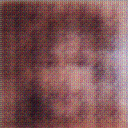
\includegraphics[width=150px]{500_fake_images/samples_5_187.png}%
\caption{A Close Up Of A Person 'S Reflection In A Mirror}%
\end{figure}

%
\end{document}